\documentclass[11pt]{article}

\usepackage[a4paper,margin=1in]{geometry}
\usepackage{amsmath,amssymb,amsthm,mathtools,bm}
\usepackage{enumitem}
\usepackage{booktabs,tabularx,array}
\usepackage{microtype}
\usepackage[hidelinks]{hyperref}
\usepackage{tikz}
\usetikzlibrary{arrows.meta,positioning,shapes.geometric}

\newtheorem{assumption}{Assumption}[section]
\newtheorem{definition}[assumption]{Definition}
\newtheorem{proposition}[assumption]{Proposition}
\newtheorem{theorem}[assumption]{Theorem}
\newtheorem{lemma}[assumption]{Lemma}
\newtheorem{corollary}[assumption]{Corollary}
\theoremstyle{remark}
\newtheorem{remark}[assumption]{Remark}
\newtheorem{example}[assumption]{Example}

\newcommand{\Hh}{H}
\newcommand{\E}{\mathbb E}
\newcommand{\Pp}{\mathbb P}
\newcommand{\R}{\mathbb R}
\newcommand{\N}{\mathbb N}
\newcommand{\Law}{\mathcal L}
\newcommand{\Lop}{\mathcal L}
\newcommand{\Cov}{\operatorname{Cov}}
\newcommand{\Var}{\operatorname{Var}}
\newcommand{\Ran}{\operatorname{Ran}}
\newcommand{\Ker}{\operatorname{Ker}}
\newcommand{\cl}{\operatorname{cl}}
\newcommand{\ip}[2]{\left\langle #1,#2\right\rangle_H}
\newcommand{\norm}[1]{\left\lVert #1\right\rVert}
\newcommand{\ThetaI}{\widetilde\Theta}
\newcommand{\PhiN}{\Phi}
\newcommand{\phiN}{\phi}
\newcommand{\obs}{\mathrm{obs}}
\newcommand{\tar}{\mathrm{tar}}
\newcommand{\diag}{\operatorname{diag}}
\newcommand{\1}{\mathbf 1}

\title{Work Package 2: Target-Specific Identification for Operator-Intervention SPDEs\\
\large Corrected theorem package, sharp conditions, and counterexamples}
\author{}
\date{5 July 2026}

\begin{document}
\maketitle

\begin{abstract}
This note establishes identification of counterfactual field-functional laws for the diagonal linear parabolic SPDE developed in Work Package~1.  The main positive result is finite-sample and exact: with known spectral geometry, noise shape, and deterministic initial condition, one stochastically excited Fourier mode observed at three equally spaced grid points identifies the diffusivity and common noise scale.  With only one positive-time observation, identification is characterised exactly by either a non-zero observed initial coefficient or variation in observed eigenvalues.  The post-intervention law at a fixed operator value depends on the factual model only through the invariant noise scale, which yields a sharper target-specific theorem than full parameter identification.  Additive measurement error is treated by deconvolution and by explicit Gaussian covariance identities.  An operator-level kernel criterion separates deterministic observability from covariance identification, and a diagonal nuisance enlargement proves the exact support condition under which unobserved modal amplitudes destroy target identification.  The note also corrects two tempting but false claims: unobserved target modes are not a problem in the scalar parametric core once the global parameters are identified, and a target mode with zero stochastic forcing is deterministic rather than unidentified when its initial contribution is known.
\end{abstract}

\section{Positive model and counterfactual target}

Let $H=L^2(D)$ and let $A_0$ be self-adjoint, negative, and have compact resolvent.  Write
\[
 A_0e_k=-\lambda_ke_k,
 \qquad 0<\lambda_1\le \lambda_2\le\cdots,
\]
for an orthonormal eigenbasis $(e_k)_{k\ge1}$.  Let
\[
 Q^{1/2}e_k=q_ke_k,
 \qquad q_k\ge0.
\]
The factual parameter is
\[
 \vartheta=(\theta,\sigma)\in
 [\underline\theta,\overline\theta]
 \times[\underline\sigma,\overline\sigma]
 \Subset(0,\infty)^2.
\]
The factual field satisfies
\begin{equation}\label{eq:factual-spde}
 dU_t=\theta A_0U_t\,dt+\sigma Q^{1/2}\,dW_t,
 \qquad U_0=u_0,
\end{equation}
where $u_0\in H$ is deterministic and known.  Its modal coordinates are independent Ornstein--Uhlenbeck processes,
\begin{equation}\label{eq:modal-factual}
 du_k(t)=-\theta\lambda_ku_k(t)\,dt+\sigma q_k\,d\beta_k(t),
 \qquad u_k(0)=u_{0,k}.
\end{equation}

For a fixed intervention value $\widetilde\theta\in\ThetaI\Subset(0,\infty)$, Work Package~1 defines
\begin{equation}\label{eq:cf-spde}
 dU_t^{\widetilde\theta}
 =\widetilde\theta A_0U_t^{\widetilde\theta}\,dt
 +\sigma Q^{1/2}\,dW_t,
 \qquad U_0^{\widetilde\theta}=u_0.
\end{equation}
For $w\in L^2(0,T;H)$, set
\[
 \Psi_w(U)=\int_0^T\ip{w_t}{U_t}\,dt,
 \qquad w_k(t)=\ip{w_t}{e_k}.
\]

\begin{assumption}[Finite target variance]\label{ass:target}
For every target $(\widetilde\theta,w)$ considered below,
\[
 V_{\widetilde\theta,w}^0
 :=\sum_{k\ge1}q_k^2\int_0^T
 \left(\int_s^T e^{-\widetilde\theta\lambda_k(t-s)}w_k(t)\,dt\right)^2ds
 <\infty.
\]
This is implied by the baseline Hilbert-space summability used in Work Package~1 together with the stated $L^2$ condition on $w$.
\end{assumption}

\begin{proposition}[Gaussian counterfactual law]\label{prop:gaussian-target}
Define
\begin{align}
 m_{\widetilde\theta,w}
 &:=\sum_{k\ge1}u_{0,k}\int_0^T
 e^{-\widetilde\theta\lambda_kt}w_k(t)\,dt,\label{eq:target-mean}\\
 g_{k,s}^{\widetilde\theta,w}
 &:=\int_s^T e^{-\widetilde\theta\lambda_k(t-s)}w_k(t)\,dt.\label{eq:gks}
\end{align}
Then
\begin{equation}\label{eq:target-law}
 \Psi_w(U^{\widetilde\theta})
 \sim\mathcal N\left(
 m_{\widetilde\theta,w},
 \sigma^2V_{\widetilde\theta,w}^0
 \right).
\end{equation}
Consequently,
\begin{equation}\label{eq:target-cdf}
 F_{\widetilde\theta,w}(z;\vartheta)
 =\PhiN\left(
 \frac{z-m_{\widetilde\theta,w}}
 {\sigma\sqrt{V_{\widetilde\theta,w}^0}}
 \right)
\end{equation}
when $V_{\widetilde\theta,w}^0>0$, with the evident point-mass formula when $V_{\widetilde\theta,w}^0=0$.
\end{proposition}

\begin{proof}
Insert the mild modal representation of \eqref{eq:cf-spde} into $\Psi_w$, apply stochastic Fubini, and obtain
\[
 \Psi_w(U^{\widetilde\theta})
 =m_{\widetilde\theta,w}
 +\sigma\sum_{k\ge1}q_k\int_0^T
 g_{k,s}^{\widetilde\theta,w}\,d\beta_k(s).
\]
The stochastic term is centred Gaussian.  Independence of the Brownian coordinates and It\^o isometry give the displayed variance.
\end{proof}

\paragraph{Identification consequence.}
For a fixed operator intervention $do(\theta=\widetilde\theta)$, the factual drift parameter $\theta$ does not appear in \eqref{eq:target-law}.  It has been overwritten.  The factual data matter through identification of the structurally invariant scale $\sigma$.  This is different from a factual-versus-counterfactual distributional effect, whose factual component generally depends on both $\theta$ and $\sigma$.

\section{Identification as constancy on observational fibres}

\begin{definition}[Observational and target equivalence]\label{def:equivalence}
Let $P_\vartheta^Y$ denote the factual observed-data law under $\vartheta$.  Define
\[
 \vartheta_1\sim_{\obs}\vartheta_2
 \quad\Longleftrightarrow\quad
 P_{\vartheta_1}^Y=P_{\vartheta_2}^Y.
\]
For a law-valued target $T(\vartheta)$, define
\[
 \vartheta_1\sim_T\vartheta_2
 \quad\Longleftrightarrow\quad
 T(\vartheta_1)=T(\vartheta_2).
\]
The target is point identified from the observed law if every observational equivalence class is contained in a target equivalence class.
\end{definition}

\begin{theorem}[Necessary and sufficient fibre criterion]\label{thm:fibre}
A target $T$ is point identified from the observed law if and only if
\begin{equation}\label{eq:fibre-criterion}
 \vartheta_1\sim_{\obs}\vartheta_2
 \quad\Longrightarrow\quad
 \vartheta_1\sim_T\vartheta_2.
\end{equation}
Equivalently, $T$ is constant on every fibre of the observation map
$\vartheta\mapsto P_\vartheta^Y$.
\end{theorem}

\begin{proof}
If $T$ is identified, two parameter values inducing the same observed law must yield the same uniquely determined target.  Conversely, if \eqref{eq:fibre-criterion} holds, define the target at an observed law by choosing any parameter value in its fibre.  Constancy on fibres makes the definition independent of the choice.
\end{proof}

\begin{remark}[Why the logical theorem is not enough]
Theorem~\ref{thm:fibre} is exact but abstract.  The remaining results compute the observational fibres for the actual spectral experiment and then evaluate the counterfactual law on those fibres.  This is the substantive identification step required by the paper.
\end{remark}

\section{Exact discrete spectral observations}

Fix $\Delta>0$, observation times $t_j=j\Delta$, $j=0,\ldots,n$, and a finite non-empty observed set $I\subset\N$.  The exact spectral data are
\[
 Y_{k,j}=u_k(t_j),
 \qquad k\in I,
 \quad j=0,\ldots,n.
\]
For each $k$, define
\begin{align}
 \rho_k(\theta)&:=e^{-\theta\lambda_k\Delta},\label{eq:rho}\\
 h_k(\theta)&:=\frac{1-e^{-2\theta\lambda_k\Delta}}
 {2\theta\lambda_k}.\label{eq:hk}
\end{align}
Then
\begin{equation}\label{eq:transition}
 Y_{k,j+1}\mid Y_{k,j}
 \sim\mathcal N\left(
 \rho_k(\theta)Y_{k,j},
 \sigma^2q_k^2h_k(\theta)
 \right).
\end{equation}
The modes are independent.

\begin{lemma}[Strict spectral-ratio monotonicity]\label{lem:ratio}
Let $0<\lambda_a<\lambda_b$ and define
\[
 R_{a,b}(\theta)
 :=\frac{h_{\lambda_a}(\theta)}{h_{\lambda_b}(\theta)},
 \qquad
 h_\lambda(\theta)
 :=\frac{1-e^{-2\theta\lambda\Delta}}
 {2\theta\lambda}.
\]
Then $R_{a,b}$ is strictly increasing on $(0,\infty)$.
\end{lemma}

\begin{proof}
Set $x=2\theta\Delta$ and $f(y)=(1-e^{-y})/y$, so $h_\lambda(\theta)=\Delta f(x\lambda)$.  Direct differentiation gives
\[
 \frac{d}{dx}\log f(x\lambda)
 =\frac{\lambda}{e^{x\lambda}-1}-\frac1x.
\]
Hence
\[
 \frac{d}{dx}\log R_{a,b}
 =\frac{\lambda_a}{e^{x\lambda_a}-1}
 -\frac{\lambda_b}{e^{x\lambda_b}-1}>0,
\]
because $\lambda\mapsto\lambda/(e^{x\lambda}-1)$ is strictly decreasing for every $x>0$.
\end{proof}

\begin{theorem}[Exact finite-sample identification]\label{thm:exact-id}
Assume $q_k>0$ for every $k\in I$ and that $\lambda_k,q_k,u_{0,k}$ are known.

\begin{enumerate}[label=\textup{(\roman*)},leftmargin=2.6em]
\item If $n\ge2$, then $(\theta,\sigma)$ is identified from the joint law of the observations as soon as $I$ contains one mode.

\item If $n=1$, then $(\theta,\sigma)$ is identified if and only if at least one of the following holds:
\begin{enumerate}[label=\textup{(\alph*)},leftmargin=2.4em]
\item $u_{0,k}\ne0$ for some $k\in I$;
\item the set $\{\lambda_k:k\in I\}$ contains at least two distinct eigenvalues.
\end{enumerate}
If all observed initial coefficients vanish and all observed eigenvalues coincide, the pair is not identified.
\end{enumerate}
\end{theorem}

\begin{proof}
For part~(i), choose any $k\in I$ and write $V_{k,1}=\Var(Y_{k,1})$.  Since $q_k,\sigma>0$, $V_{k,1}>0$.  The Markov recursion gives
\[
 \Cov(Y_{k,1},Y_{k,2})=\rho_k(\theta)V_{k,1}.
\]
Thus the joint law identifies
\begin{equation}\label{eq:rho-from-cov}
 \rho_k(\theta)
 =\frac{\Cov(Y_{k,1},Y_{k,2})}
 {\Var(Y_{k,1})}.
\end{equation}
Strict monotonicity of $\theta\mapsto e^{-\theta\lambda_k\Delta}$ identifies
\[
 \theta=-\frac{\log\rho_k}{\lambda_k\Delta}.
\]
Then
\begin{equation}\label{eq:sigma-from-var}
 \sigma^2
 =\frac{\Var(Y_{k,1})}{q_k^2h_k(\theta)}
\end{equation}
identifies $\sigma$.

For part~(ii), the one-step mean and variance are
\[
 \E Y_{k,1}=\rho_k(\theta)u_{0,k},
 \qquad
 \Var(Y_{k,1})=\sigma^2q_k^2h_k(\theta).
\]
If some $u_{0,k}\ne0$, the mean identifies $\rho_k$ and hence $\theta$; the variance then identifies $\sigma$.  If all observed initial coefficients vanish but two distinct eigenvalues are observed, the law identifies the variance ratio
\[
 \frac{\Var(Y_{a,1})/q_a^2}
 {\Var(Y_{b,1})/q_b^2}
 =\frac{h_a(\theta)}{h_b(\theta)},
\]
and Lemma~\ref{lem:ratio} identifies $\theta$, followed by $\sigma$.

Conversely, if all observed initial coefficients vanish and all observed eigenvalues equal a common value $\lambda_\star$, the joint law depends on $(\theta,\sigma)$ only through
\[
 c=\sigma^2h_{\lambda_\star}(\theta).
\]
For any $\theta_2\ne\theta_1$, choosing
\[
 \sigma_2^2=\sigma_1^2
 \frac{h_{\lambda_\star}(\theta_1)}
 {h_{\lambda_\star}(\theta_2)}
\]
produces the same observed law.  The pair is therefore not identified.
\end{proof}

\begin{remark}[The conditional-kernel shortcut]
Equality of the formal transition kernels for all possible current states would identify $\theta$ from the conditional mean coefficient.  The experiment, however, observes a joint law from one fixed initial condition.  Theorem~\ref{thm:exact-id} states the conditions under which that actual joint law identifies the parameters; it does not silently replace the data by an oracle that reveals the transition kernel at every state.
\end{remark}

\section{Target-specific identification in the scalar core}

\begin{theorem}[Sharp identification of the fixed-intervention law]\label{thm:target-specific}
Fix $(\widetilde\theta,w)$ and write $m=m_{\widetilde\theta,w}$ and $V^0=V_{\widetilde\theta,w}^0$.

\begin{enumerate}[label=\textup{(\roman*)},leftmargin=2.6em]
\item If $V^0=0$, the counterfactual law is the known point mass $\delta_m$ and is identified without identifying either $\theta$ or $\sigma$.

\item If $V^0>0$, the full counterfactual law is identified if and only if $\sigma$ is constant on every observational equivalence class.

\item If $V^0>0$ and only the scalar CDF ordinate $F_{\widetilde\theta,w}(z)$ is targeted, then:
\begin{enumerate}[label=\textup{(\alph*)},leftmargin=2.4em]
\item at $z=m$, the ordinate equals $1/2$ for every $\sigma>0$ and is therefore identified even when $\sigma$ is not;
\item at every $z\ne m$, the ordinate is identified if and only if $\sigma$ is constant on every observational equivalence class.
\end{enumerate}
\end{enumerate}
\end{theorem}

\begin{proof}
Part~(i) follows from Proposition~\ref{prop:gaussian-target}.  For part~(ii), Gaussian laws with the same known mean $m$ are equal exactly when their positive variances $\sigma^2V^0$ are equal.  Because $V^0$ is known and positive, this is equivalent to equality of $\sigma$.  For part~(iii), use \eqref{eq:target-cdf}.  At $z=m$ the argument of $\PhiN$ is zero.  For $z\ne m$, the map $\sigma\mapsto\PhiN((z-m)/(\sigma\sqrt{V^0}))$ is strictly monotone on $(0,\infty)$.
\end{proof}

\begin{corollary}[Identification under exact spectral sampling]\label{cor:target-exact}
Under any condition in Theorem~\ref{thm:exact-id} that identifies $\sigma$, every fixed-intervention field-functional law satisfying Assumption~\ref{ass:target} is identified, including targets with Fourier support outside the observed set $I$.
\end{corollary}

\begin{remark}[Why unobserved target modes do not fail in the core]
The covariance shape $Q$, all eigenvalues, and the common scale structure $\sigma^2Q$ are known up to the single scalar $\sigma^2$.  Once one observed mode identifies that scalar, the stochastic contribution of every unobserved mode is determined.  The support condition $I_{\tar}(w)\subseteq I_{\obs}$ becomes necessary only in a larger model where unobserved modal amplitudes are free nuisance parameters; Section~\ref{sec:modal-nuisance} proves that result.
\end{remark}

\begin{remark}[Factual-versus-counterfactual effects]
The law under a fixed $do(\theta=\widetilde\theta)$ depends on the factual parameter only through $\sigma$.  By contrast, a distributional effect
\[
 F_{\widetilde\theta,w}(z;\vartheta)
 -F_{\theta,w}(z;\vartheta)
\]
contains a factual law whose semigroup is indexed by the unknown $\theta$.  Except in degenerate cases, identification of that effect requires both $\theta$ and $\sigma$.
\end{remark}

\section{Noisy spectral observations}

Suppose now that
\begin{equation}\label{eq:noisy-obs}
 Z_{k,j}=Y_{k,j}+\varepsilon_{k,j},
\end{equation}
where the measurement errors are independent of the state process.

\begin{proposition}[Known-error deconvolution]\label{prop:deconv}
Fix a finite observed vector $Y$ and suppose the additive error vector $\varepsilon$ has a known distribution, is independent of $Y$, and has a characteristic function that is nowhere zero.  Then the law of $Y$ is identified from the law of $Z=Y+\varepsilon$.  Consequently, every identification result for exact spectral observations transfers to this noisy experiment.
\end{proposition}

\begin{proof}
Independence gives
\[
 \varphi_Z(t)=\varphi_Y(t)\varphi_\varepsilon(t).
\]
Since $\varphi_\varepsilon$ is known and never vanishes,
$\varphi_Y=\varphi_Z/\varphi_\varepsilon$ is uniquely determined.  Characteristic functions determine probability laws.
\end{proof}

\begin{theorem}[Explicit Gaussian measurement-error identification]\label{thm:noisy-gaussian}
Observe one mode $k$ with $q_k>0$ at equally spaced times and let
\[
 Z_j=Y_{k,j}+\varepsilon_j,
 \qquad
 \varepsilon_j\overset{\mathrm{iid}}{\sim}\mathcal N(0,r),
\]
independently of the state.

\begin{enumerate}[label=\textup{(\roman*)},leftmargin=2.6em]
\item If $r$ is known and $n\ge2$, then $(\theta,\sigma)$ is identified.
\item If $r$ is unknown and $n\ge3$, then $(\theta,\sigma,r)$ is identified.
\end{enumerate}
\end{theorem}

\begin{proof}
Let $V_1=\Var(Y_{k,1})>0$ and $\rho=e^{-\theta\lambda_k\Delta}$.
If $r$ is known,
\[
 V_1=\Var(Z_1)-r,
 \qquad
 \Cov(Z_1,Z_2)=\rho V_1,
\]
so $\rho$, then $\theta$, then $\sigma$ are identified as in \eqref{eq:sigma-from-var}.

If $r$ is unknown, measurement error does not affect cross-time covariances and
\[
 \Cov(Z_1,Z_2)=\rho V_1,
 \qquad
 \Cov(Z_1,Z_3)=\rho^2V_1.
\]
Therefore
\[
 \rho=
 \frac{\Cov(Z_1,Z_3)}{\Cov(Z_1,Z_2)},
 \qquad
 V_1=\frac{\Cov(Z_1,Z_2)}{\rho}.
\]
This identifies $\theta$ and $\sigma$, and finally
$r=\Var(Z_1)-V_1$.
\end{proof}

\begin{remark}[Scope of the moment argument]
The theorem uses temporally independent measurement noise and equal sampling intervals.  Correlated errors, unknown error dynamics, or intervention-dependent measurement require a different state-space identification analysis.  The general linear-Gaussian literature also warns that unrestricted process-noise, measurement-noise, and unknown-input structures need not be jointly identifiable without additional restrictions.
\end{remark}

\section{Operator-level identification under partial observation}\label{sec:operator}

This section states the correct infinite-dimensional principle.  It shows why a deterministic observable-subspace condition is exact for the mean but is not, by itself, a complete covariance-identification theorem.

Let $S_\theta(t)=e^{t\theta A_0}$ be fixed and let $\mathcal H:H\to Y$ be a bounded observation operator into a Hilbert space $Y$.  Consider a Gaussian model indexed by a deterministic initial state $u$ and a positive trace-class noise covariance $C$:
\[
 dU_t=\theta A_0U_t\,dt+C^{1/2}\,dW_t,
 \qquad U_0=u,
 \qquad Y_t=\mathcal HU_t.
\]
Define the factual mean and covariance maps
\begin{align}
 (\mathfrak M_\theta u)(t)
 &:=\mathcal H S_\theta(t)u,\label{eq:M-map}\\
 (\mathfrak K_\theta C)(t,r)
 &:=\int_0^{t\wedge r}
 \mathcal H S_\theta(t-s)C
 S_\theta(r-s)^*\mathcal H^*\,ds.\label{eq:K-map}
\end{align}
For a counterfactual target, define
\begin{align}
 r_0^{\widetilde\theta,w}
 &:=\int_0^T S_{\widetilde\theta}(t)^*w_t\,dt,\label{eq:r0}\\
 g_s^{\widetilde\theta,w}
 &:=\int_s^T S_{\widetilde\theta}(t-s)^*w_t\,dt,\label{eq:gs-abstract}\\
 \mathfrak L_{\widetilde\theta,w}(u)
 &:=\ip{r_0^{\widetilde\theta,w}}{u},\label{eq:L-map}\\
 \mathfrak V_{\widetilde\theta,w}(C)
 &:=\int_0^T\ip{C g_s^{\widetilde\theta,w}}{g_s^{\widetilde\theta,w}}\,ds.\label{eq:V-map}
\end{align}

\begin{theorem}[Kernel characterisation for Gaussian partial observation]\label{thm:operator-kernel}
Let the admissible model class be a product $\mathcal U\times\mathcal C$, where $\mathcal U\subset H$ and $\mathcal C$ is a convex class of positive trace-class operators.  The counterfactual Gaussian law is identified from the complete factual output law if and only if
\begin{align}
 \Ker(\mathfrak M_\theta)\cap(\mathcal U-\mathcal U)
 &\subseteq\Ker(\mathfrak L_{\widetilde\theta,w}),\label{eq:mean-kernel}\\
 \Ker(\mathfrak K_\theta)\cap(\mathcal C-\mathcal C)
 &\subseteq\Ker(\mathfrak V_{\widetilde\theta,w}).\label{eq:cov-kernel}
\end{align}
Moreover, if
\[
 \mathcal O_\theta
 :=\overline{\operatorname{span}}
 \{S_\theta(t)^*\mathcal H^*y:
 t\in[0,T],\ y\in Y\},
\]
then the unrestricted mean condition \eqref{eq:mean-kernel} is equivalent to
\begin{equation}\label{eq:r-in-O}
 r_0^{\widetilde\theta,w}\in\mathcal O_\theta.
\end{equation}
\end{theorem}

\begin{proof}
A Gaussian output law is determined by its mean and covariance.  Equality of output means for $u_1,u_2$ is equivalent to
$u_1-u_2\in\Ker(\mathfrak M_\theta)$; equality of output covariances for $C_1,C_2$ is equivalent to
$C_1-C_2\in\Ker(\mathfrak K_\theta)$.  The counterfactual Gaussian laws agree exactly when the target means and variances agree.  This proves the two kernel conditions.

For the final statement,
\[
 \Ker(\mathfrak M_\theta)
 =\mathcal O_\theta^\perp.
\]
A continuous linear functional $u\mapsto\ip{r_0}{u}$ vanishes on
$\mathcal O_\theta^\perp$ if and only if $r_0\in\mathcal O_\theta$.
\end{proof}

\begin{remark}[Covariance observability is a lifted problem]
The inclusion $g_s^{\widetilde\theta,w}\in\mathcal O_\theta$ is a useful sufficient ingredient only when the factual output law actually identifies the covariance bilinear form on that subspace.  In general, covariance identification concerns the lifted operator map $\mathfrak K_\theta$ on trace-class operators, not merely the state-space observability subspace.  The exact criterion is \eqref{eq:cov-kernel}.  The diagonal result below computes that kernel explicitly.
\end{remark}

\section{Exact modal-support theorem in a nuisance enlargement}\label{sec:modal-nuisance}

To make the observable-support boundary substantive, enlarge the scalar core to
\begin{equation}\label{eq:modal-nuisance}
 du_k(t)=-a_ku_k(t)\,dt+b_k\,d\beta_k(t),
 \qquad b_k\ge0,
\end{equation}
with mode-specific invariant amplitudes $b_k$.  Suppose exact spectral data identify $(a_k,b_k)$ for every observed mode $k\in I_{\obs}$.  Let $J_{\mathrm{free}}$ be the set of unobserved modes whose amplitudes are not otherwise known.  Under intervention, the drift of mode $k$ is replaced by a known $\widetilde a_k>0$, while $b_k$ is preserved.

Define
\begin{equation}\label{eq:Bk}
 B_k(w):=\int_0^T
 \left(\int_s^T e^{-\widetilde a_k(t-s)}w_k(t)\,dt\right)^2ds.
\end{equation}
The counterfactual variance is $\sum_kb_k^2B_k(w)$.

\begin{lemma}[Effective support]\label{lem:effective-support}
For $\widetilde a_k>0$, $B_k(w)=0$ if and only if $w_k=0$ in $L^2(0,T)$.
\end{lemma}

\begin{proof}
Let
$g(s)=\int_s^T e^{-\widetilde a_k(t-s)}w_k(t)\,dt$.
Then $g$ is absolutely continuous, $g(T)=0$, and
$g'(s)=\widetilde a_kg(s)-w_k(s)$ almost everywhere.  If $B_k(w)=\norm{g}_{L^2}^2=0$, then $g=0$ almost everywhere and therefore $w_k=0$ almost everywhere.  The converse is immediate.
\end{proof}

\begin{theorem}[Sharp diagonal target-support condition]\label{thm:support}
In model \eqref{eq:modal-nuisance}, assume the admissible class permits each $b_k^2$, $k\in J_{\mathrm{free}}$, to vary over a non-degenerate interval independently of the observed parameters.  Then the counterfactual field-functional law is identified if and only if
\begin{equation}\label{eq:support-condition}
 B_k(w)=0
 \quad\text{for every }k\in J_{\mathrm{free}}\setminus I_{\obs}.
\end{equation}
Equivalently,
\[
 I_{\tar}(w)\cap J_{\mathrm{free}}
 \subseteq I_{\obs},
 \qquad
 I_{\tar}(w):=\{k:w_k\ne0\text{ in }L^2(0,T)\}.
\]
Unobserved modes with structurally known amplitudes need not belong to $I_{\obs}$.
\end{theorem}

\begin{proof}
For observed modes and structurally known unobserved modes, every term $b_k^2B_k(w)$ is identified.  If \eqref{eq:support-condition} holds, all remaining free unobserved terms vanish, so the target variance and hence the Gaussian law are identified.

Conversely, suppose $B_\ell(w)>0$ for some free unobserved mode $\ell$.  Change $b_\ell^2$ while holding every observed parameter and every other structural component fixed.  The factual observed law is unchanged because mode $\ell$ is not observed, while the target variance changes by
$\Delta b_\ell^2B_\ell(w)\ne0$.  The target law is not identified.
\end{proof}

\begin{remark}[Parametric linkage versus modal freedom]
Theorem~\ref{thm:support} does not contradict Corollary~\ref{cor:target-exact}.  In the scalar core, $b_k=\sigma q_k$ and known $q_k$ link every modal amplitude to one identified scalar.  In the nuisance enlargement, unobserved $b_k$ may vary independently, and support becomes decisive.
\end{remark}

\section{Heat-equation corollary}

\begin{corollary}[Dirichlet stochastic heat equation]\label{cor:heat}
Let $D=(0,1)$, $A_0=\Delta$ with Dirichlet boundary conditions,
\[
 e_k(x)=\sqrt2\sin(k\pi x),
 \qquad
 \lambda_k=\pi^2k^2,
\]
and suppose $q_k>0$ is known for at least one observed mode $k$.  Exact observation of that coefficient at times $0,\Delta,2\Delta$ identifies
\begin{align}
 \rho_k&=
 \frac{\Cov(Y_{k,1},Y_{k,2})}{\Var(Y_{k,1})},\\
 \theta&=-\frac{\log\rho_k}{\pi^2k^2\Delta},\\
 \sigma^2&=
 \frac{2\theta\pi^2k^2\Var(Y_{k,1})}
 {q_k^2(1-\rho_k^2)}.
\end{align}
Therefore every fixed-intervention law
$\Law(\Psi_w(U^{\widetilde\theta}))$ with finite variance is identified, regardless of whether $w$ uses Fourier modes not directly observed.
\end{corollary}

\section{Sharp counterexamples and corrected failure catalogue}

\begin{example}[One time, one zero-start mode]\label{ex:one-time}
Observe one mode at $t=\Delta$ with $u_{0,k}=0$.  The observed law is
\[
 Y_{k,1}\sim\mathcal N(0,\sigma^2q_k^2h_k(\theta)).
\]
For every $\theta_2\ne\theta_1$, rescale $\sigma_2$ as in the proof of Theorem~\ref{thm:exact-id}.  The observed law is unchanged.  A non-degenerate fixed-intervention target changes because its variance is proportional to $\sigma^2$.  Thus causal semantics does not imply identification.
\end{example}

\begin{example}[Invisible modal nuisance]\label{ex:invisible}
In the two-mode nuisance model, observe only mode~1 and target a functional supported on mode~2.  Two models differing only in $b_2$ have identical factual observations and different counterfactual variances.  This is the canonical rank-deficient-sensing failure.
\end{example}

\begin{example}[Unknown measurement variance with insufficient lags]\label{ex:measurement}
With one noisy positive-time observation and $u_{0,k}=0$,
\[
 \Var(Z_1)=\sigma^2q_k^2h_k(\theta)+r.
\]
Many triples $(\theta,\sigma,r)$ give the same law.  More temporal covariance information or known error structure is necessary.
\end{example}

\begin{example}[Unknown observation scale]\label{ex:unknown-H}
If the scalar observation is $Z_j=cY_j$ with unknown $c>0$, then only products such as $c\sigma$ are identified from centred second moments.  A target for the latent field, rather than the scaled observation, is not identified without normalising or otherwise identifying $c$.
\end{example}

\begin{example}[Intervention-dependent measurement]\label{ex:intervention-measurement}
A factual law generated through $\mathcal H$ contains no information about an unrestricted post-intervention operator $\widetilde{\mathcal H}$.  Replacing the dynamics and measurement simultaneously is a different intervention and requires a separate invariance or identification assumption.
\end{example}

\begin{remark}[Zero forcing is not automatically non-identification]
If $q_k=0$ on a target mode and $u_{0,k}$ is known, that modal target contribution is deterministic and known.  Non-identification arises only if another unknown component, such as the initial coefficient or deterministic forcing, remains free.  Accordingly, ``$q_k=0$ on a target mode'' is not a valid negative theorem for the present positive core.
\end{remark}

\begin{remark}[Unknown forcing]
An unrestricted deterministic or adapted forcing can offset changes in the drift operator and reproduce factual observations while altering post-intervention behaviour.  The full construction belongs to the dedicated non-identification work package; WP2 records it as a boundary, not as part of the positive model.
\end{remark}

\section{Identification DAG}

\begin{center}
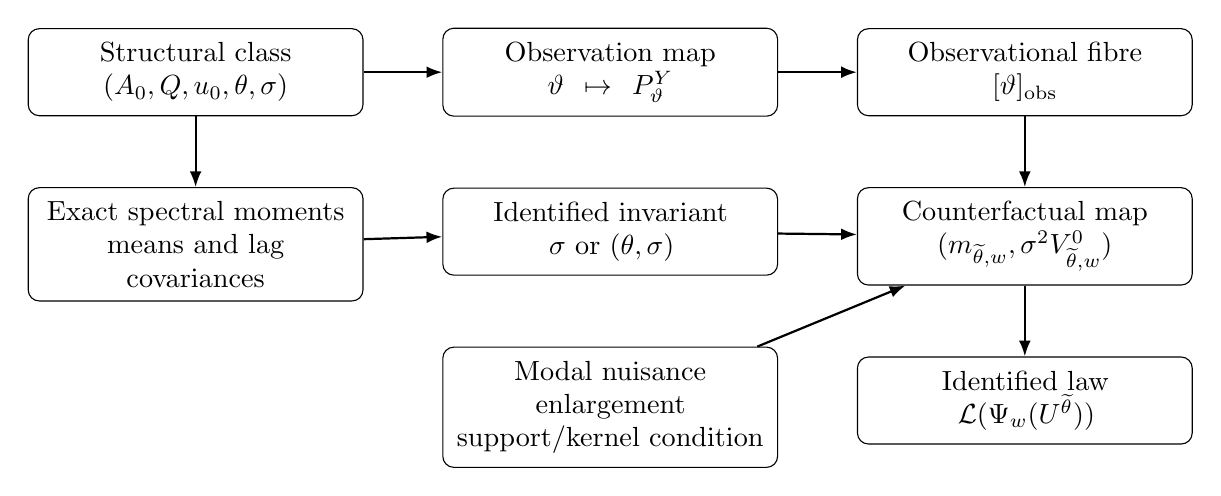
\begin{tikzpicture}[
 node distance=9mm and 10mm,
 box/.style={draw,rounded corners,align=center,inner sep=5pt,text width=39mm},
 arr/.style={-{Latex[length=2mm]},thick}
]
\node[box] (struct) {Structural class\\$(A_0,Q,u_0,\theta,\sigma)$};
\node[box,right=of struct] (obsmap) {Observation map\\$\vartheta\mapsto P_\vartheta^Y$};
\node[box,right=of obsmap] (fibre) {Observational fibre\\$[\vartheta]_{\obs}$};

\node[box,below=of struct] (exact) {Exact spectral moments\\means and lag covariances};
\node[box,below=of obsmap] (params) {Identified invariant\\$\sigma$ or $(\theta,\sigma)$};
\node[box,below=of fibre] (target) {Counterfactual map\\$(m_{\widetilde\theta,w},\sigma^2V^0_{\widetilde\theta,w})$};

\node[box,below=of params] (nuisance) {Modal nuisance enlargement\\support/kernel condition};
\node[box,below=of target] (law) {Identified law\\$\Law(\Psi_w(U^{\widetilde\theta}))$};

\draw[arr] (struct) -- (obsmap);
\draw[arr] (obsmap) -- (fibre);
\draw[arr] (struct) -- (exact);
\draw[arr] (exact) -- (params);
\draw[arr] (fibre) -- (target);
\draw[arr] (params) -- (target);
\draw[arr] (nuisance) -- (target);
\draw[arr] (target) -- (law);
\end{tikzpicture}
\end{center}

\section{Assumptions, conclusions, and failure modes}

\renewcommand{\arraystretch}{1.18}
\begin{tabularx}{\textwidth}{>{\raggedright\arraybackslash}p{0.23\textwidth} X X}
\toprule
Setting & Identification conclusion & Principal failure mode \\
\midrule
Exact, one excited mode, $n\ge2$ & $(\theta,\sigma)$ and all fixed-intervention laws are identified & No excited observed mode \\
Exact, one step & Identified iff a non-zero observed initial coefficient or two distinct observed eigenvalues are available & Zero starts and one repeated eigenvalue reveal only $\sigma^2h_\lambda(\theta)$ \\
Known additive error, non-vanishing characteristic function & Latent finite-dimensional law is recovered by deconvolution & Unknown or vanishing error characteristic function \\
Gaussian error, known variance, $n\ge2$ & $(\theta,\sigma)$ identified from variance and lag covariance & Correlated or misspecified error \\
Gaussian error, unknown variance, $n\ge3$ & $(\theta,\sigma,r)$ identified from two off-diagonal covariances & Too few lags \\
Scalar parametric core & Unobserved target modes are identified once $\sigma$ is identified & Unknown $Q$ shape or broken common-scale restriction \\
Mode-specific nuisance amplitudes & Target identified iff every free unobserved target coefficient vanishes & Invisible free modal amplitude \\
General partial observation & Kernel inclusions \eqref{eq:mean-kernel}--\eqref{eq:cov-kernel} are necessary and sufficient & Covariance map has target-relevant null directions \\
\bottomrule
\end{tabularx}

\section{WP2 completion statement}

The positive identification step is now explicit rather than assumed.  The exact spectral experiment identifies the structural parameters under finite-sample conditions stated in Theorem~\ref{thm:exact-id}.  Theorem~\ref{thm:target-specific} then states precisely which part of that identification is needed for a fixed operator intervention.  The operator kernel theorem supplies the correct general abstraction, while Theorem~\ref{thm:support} gives a sharp observable-support result in the modal nuisance model.  The noisy-observation results and counterexamples delimit the extension without conflating theoretical identification with estimation quality.

\section*{Literature position}

Spectral observation is a standard and especially tractable experiment in statistical inference for parabolic SPDEs.  Linear-Gaussian state-space representations provide the natural language for noisy discrete observations, while infinite-dimensional observability is formulated through operator semigroups.  The contribution of this work package is not a new general theory of linear-system identification.  It is the exact connection between those tools and the operator-intervention target: observational fibres are computed for the SPDE core, the invariant structural component required by the counterfactual is isolated, and the observable-support boundary is proved in a model where it is genuinely necessary.

\begin{thebibliography}{9}

\bibitem{Cialenco2018}
I.~Cialenco,
``Statistical inference for SPDEs: an overview'',
\emph{Statistical Inference for Stochastic Processes}, 21 (2018), 309--329.

\bibitem{DPZ2014}
G.~Da Prato and J.~Zabczyk,
\emph{Stochastic Equations in Infinite Dimensions}, 2nd ed.,
Cambridge University Press, 2014.

\bibitem{HannanDeistler2012}
E.~J. Hannan and M.~Deistler,
\emph{The Statistical Theory of Linear Systems},
Classics in Applied Mathematics, SIAM, 2012 reprint.

\bibitem{SarkkaSolin2019}
S.~S\"arkk\"a and A.~Solin,
\emph{Applied Stochastic Differential Equations},
Cambridge University Press, 2019.

\bibitem{TucsnakWeiss2009}
M.~Tucsnak and G.~Weiss,
\emph{Observation and Control for Operator Semigroups},
Birkh\"auser, 2009.

\end{thebibliography}

\end{document}
